% !TEX encoding = UTF-8
% !TEX TS-program = pdflatex
% !TEX root = ../tesi.tex

%**************************************************************
\chapter{Implementazione del progetto}
\label{cap:implementazione}
%**************************************************************
\section{Analisi dei requisiti}

\subsection{Attori}
Nella figura \ref{fig:attori} è riportato il diagramma \emph{\acrshort{uml}} che descrive la gerarchia degli attori del sistema. Dopo un'attenta analisi ho individuato: cinque \
attori principali e uno secondario. Gli attori principali da me individuati sono: l'utente non autenticato, l'utente non autorizzato, l'utente \
di tipo fornitore, l'utente di tipo lago e l'utente di tipo lago \emph{admin}. L'unico utente secondario che ho individuato è Google, in quanto all'interno del sistema \
utilizziamo \emph{Google SSO} come servizio di autenticazione. 

\begin{figure}[!ht]
  \begin{center}
    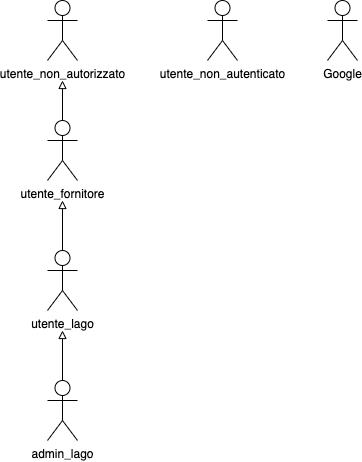
\includegraphics[scale=0.5]{usecase/attori}
    \caption{Gerarchia degli attori di sistema}
    \label{fig:attori}
  \end{center}
\end{figure}

\subsection{Casi d'uso}
Durante l'attività di analisi ho definito diversi diagrammi dei casi d'uso mediante il linguaggio \emph{\acrshort{uml}}. Tutti i diagrammi sono contenuti all'interno \
del documento di analisi aziendale. In questa sezione mostrerò solo il caso d'uso più generale per dare un'idea di ciò che è possibile fare all'interno \
dell'applicazione. Ogni caso d'uso segue la seguente denominazione:

\begin{center}
  UC[codice]
\end{center}

dove per [codice] si intende un identificativo univoco del caso d'uso riportato in forma gerarchica. Per ogni caso d'uso, inoltre, vengono specificati:
\begin{itemize}
  \item Gli attori coinvolti;
  \item Una breve descrizione;
  \item La precondizione;
  \item La postcondizione;
  \item Lo scenario principale;
  \item Le eventuali estensioni.
\end{itemize}

\subsubsection{Caso d'uso UC0 - Scenario principale}
\begin{figure}[!ht]
  \begin{center}
    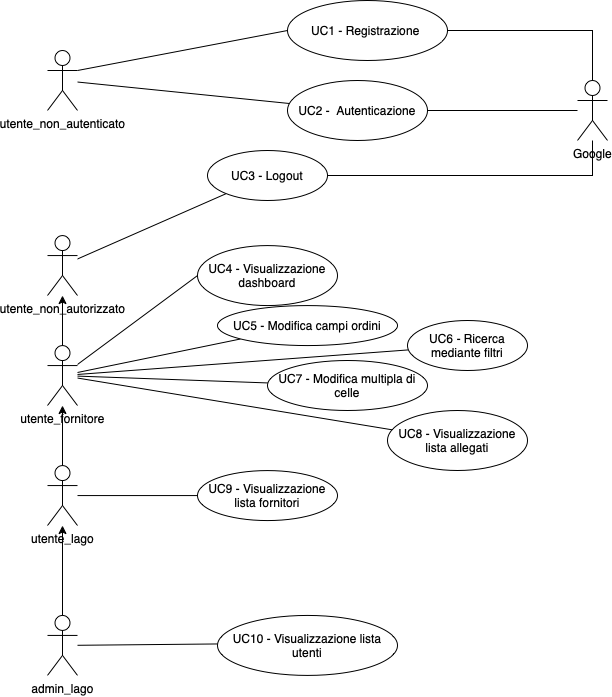
\includegraphics[scale=0.35]{usecase/main-scenario}
    \caption{UC0: Scenario principale}
    \label{fig:uc0}
  \end{center}
\end{figure}

\begin{itemize}
  \item \textbf{Attori:} utente non autenticato, utente autenticato, utente di tipo fornitore, utente di tipo lago e utente di tipo lago \emph{admin};
  \item \textbf{Descrizione:} nella schermata principale un utente non autenticato può autenticarsi, o registrarsi, tramite l'apposito pulsante che reindirizza l'utente al \emph{form} di Google. Un utente non autorizzato può effettuare il \emph{logout} dalla piattaforma. Un utente di tipo fornitore, oltre alle funzionalità dell'utente non autorizzato, ha la possibilità di:\
    \begin{itemize}
      \item visualizzare la \emph{dashboard};
      \item modificare una riga;
      \item effettuare la ricerca mediante filtri;
      \item effettuare la modifica multipla di cella;
      \item visualizzare gli allegati relativi ad un ordine.
    \end{itemize}
    Un utente di tipo lago, oltre alle funzionalità dell'utente fornitore, può visualizzare la lista dei fornitori. Un utente di tipo lago \emph{admin}, infine, oltre alle funzionalità dell'utente lago, può visualizzare la lista degli utenti registrati sulla piattaforma;
  \item \textbf{Precondizione:} il sistema è avviato e mostra la pagina principale dell'applicazione;
  \item \textbf{Postcondizione:} il sistema ha ricevuto tutte le informazioni dall'utente sulle operazioni che vuole eseguire;
  \item \textbf{Scenario principale:} 
    \begin{itemize}
      \item L'utente non autenticato può effettuare la registrazione alla piattaforma (UC1);
      \item L'utente non autenticato può effettuare l'autenticazione (UC2);
      \item L'utente non autorizzato, l'utente di tipo fornitore, l'utente di tipo lago e l'utente di tipo \emph{admin} possono effettuare il \emph{logout} (UC3);
      \item L'utente di tipo fornitore, l'utente di tipo lago e l'utente di tipo \emph{admin} possono visualizzare la \emph{dashboard} (UC4);
      \item L'utente di tipo fornitore, l'utente di tipo lago e l'utente di tipo \emph{admin} possono modificare un campo di un ordine (UC5);
      \item L'utente di tipo fornitore, l'utente di tipo lago e l'utente di tipo \emph{admin} possono effettuare la ricerca mediante filtri (UC6);
      \item L'utente di tipo fornitore, l'utente di tipo lago e l'utente di tipo \emph{admin} possono effettuare la modifica multipla di ordini (UC7);
      \item L'utente di tipo fornitore, l'utente di tipo lago e l'utente di tipo \emph{admin} possono visualizzare gli allegati di un ordine (UC8);
      \item L'utente di tipo lago e l'utente di tipo \emph{admin} possono visualizzare la lista dei fornitori (UC9);
      \item L'utente di tipo lago \emph{admin} può visualizzare la lista degli utenti registrati nella piattaforma (UC10).
    \end{itemize}
\end{itemize}

\subsection{\emph{User Stories}}
Grazie alla definizione dei casi d'uso ho estratto le \emph{user stories} che ho implementato durante il periodo di \emph{stage}. Di seguito sono riportate quelle relative alle funzionalità principali.

\subsubsection{Login con \emph{Google SSO} (5)}
Come utente non autenticato voglio poter accedere alla piattaforma mediante \emph{Google SSO}. \\
\emph{Tasks:}
\begin{itemize}
  \item \emph{\gls{backend}}:
    \begin{itemize}
      \item Creazione \emph{collection users};
      \item Implementazione chiamata \emph{\acrshort{api}} di \emph{Google SSO};
      \item Se l'utente non è presente, memorizzare il \emph{token} e metterlo in \emph{"pending"};
      \item Verifica della validità del \emph{token}.
    \end{itemize}
  \item \emph{\gls{frontend}}:
    \begin{itemize}
      \item Implementazione della chiamata all'\emph{\acrshort{api}} di \emph{login} del \emph{\gls{backend}};
      \item Creazione della sessione utente;
      \item Reindirizzamento alla \emph{dashboard}.
    \end{itemize}
\end{itemize}

\subsubsection{Visualizzazione lista fornitori (5)}
Come utente Lago voglio visualizzare la lista di tutti i fornitori abilitati. \\
\emph{Tasks:}
\begin{itemize}
  \item \emph{\gls{backend}}:
    \begin{itemize}
      \item Creazione \emph{collection suppliers};
      \item Verifica dei permessi di esecuzione dell'\emph{\acrshort{api}};
      \item Implementazione dell'\emph{\acrshort{api} "get suppliers"}.
    \end{itemize}
  \item \emph{\gls{frontend}}:
    \begin{itemize}
      \item Implementazione della chiamata all'\emph{\acrshort{api} "get suppliers"} del \emph{\gls{backend}};
      \item Visualizzazione della lista dei fornitori.
    \end{itemize}
\end{itemize}

\subsubsection{Visualizzazione fornitore (5)}
Come utente Lago o utente di tipo fornitore voglio visualizzare la griglia di un fornitore. \\
\emph{Tasks:}
\begin{itemize}
  \item \emph{\gls{backend}}:
    \begin{itemize}
      \item Definizione della struttura della configurazione di una colonna;
      \item Definizione della struttura della configurazione per il contenuto della colonna;
      \item Creazione \emph{collection order-rows};
      \item Verifica dei permessi di esecuzione dell'\emph{\acrshort{api}};
      \item Implementazione dell'\emph{\acrshort{api} "get order-rows"} di un fornitore.
    \end{itemize}
  \item \emph{\gls{frontend}}:
    \begin{itemize}
      \item Implementazione della chiamata all'\emph{\acrshort{api} "get order-rows"} del \emph{\gls{backend}};
      \item Visualizzazione della griglia con i dati degli ordini di un fornitore.
    \end{itemize}
\end{itemize}

\subsubsection{Modifica dei campi di un ordine (5)}
Come utente Lago o utente di tipo fornitore voglio poter modificare un campo di un ordine. \\
\emph{Tasks:}
\begin{itemize}
  \item \emph{\gls{backend}}:
    \begin{itemize}
      \item Verifica dei permessi di esecuzione dell'\emph{\acrshort{api}};
      \item Implementazione dell'\emph{\acrshort{api} "update order-row"} per un ordine di un fornitore.
    \end{itemize}
  \item \emph{\gls{frontend}}:
    \begin{itemize}
      \item Validazione del campo modificato;
      \item Visualizzazione di un errore in caso di valore non valido;
      \item Implementazione della chiamata all'\emph{\acrshort{api} "update order-row"} del \emph{\gls{backend}};
      \item Visualizzazione della griglia con i dati degli ordini aggiornati.
    \end{itemize}
\end{itemize}

\subsubsection{Visualizzazione della lista degli utenti (5)}
Come utente Lago \emph{admin} voglio poter visualizzare la lista degli utenti registrati. \\
\emph{Tasks:}
\begin{itemize}
  \item \emph{\gls{backend}}:
    \begin{itemize}
      \item Verifica dei permessi di esecuzione dell'\emph{\acrshort{api}};
      \item Implementazione dell'\emph{\acrshort{api} "get users"}.
    \end{itemize}
  \item \emph{\gls{frontend}}:
    \begin{itemize}
      \item Implementazione della chiamata all'\emph{\acrshort{api} "get users"} del \emph{\gls{backend}};
      \item Visualizzazione della lista degli utenti.
    \end{itemize}
\end{itemize}

\subsubsection{Visualizzazione della lista degli allegati (5)}
Come utente Lago o utente di tipo fornitore voglio poter visualizzare la lista degli allegati relativi ad un ordine. \\
\emph{Tasks:}
\begin{itemize}
  \item \emph{\gls{backend}}:
    \begin{itemize}
      \item Verifica dei permessi di esecuzione dell'\emph{\acrshort{api}};
      \item Implementazione del sistema per l'invio dei file allegati da visualizzare;
      \item Implementazione dell'\emph{\acrshort{api} "get attachments"} di un ordine.
    \end{itemize}
  \item \emph{\gls{frontend}}:
    \begin{itemize}
      \item Implementazione della chiamata all'\emph{\acrshort{api} "get attachments"} del \emph{\gls{backend}};
      \item Visualizzazione della lista degli allegati di un ordine.
    \end{itemize}
\end{itemize}

%**************************************************************
\section{Progettazione architetturale}

\subsection{Architettura di sitema}
L'applicazione è costituita da due parti principali: il \emph{\gls{frontend}} e il \emph{\gls{backend}} che costituiscono rispettivamente il \emph{client} e il \emph{server} nell'architettura \emph{client-server}. \
All'interno di questa architettura, il \emph{\gls{frontend}} ha il compito interagire con l'utente e di mostrare i dati ottenuti dal \emph{server}. Il \emph{\gls{backend}}, invece, fornisce le \emph{\acrshort{api}} \
per poter svolgere determinate operazioni e ottenerne i risultati. Entrambi i componenti sono indipendenti tra loro e comunicano utilizzando le richieste \emph{\acrshort{http}}, possono essere di diversi tipi, a \
seconda dell'operazione che intendiamo svolgere: 
\begin{itemize}
  \item \emph{GET}: per ottenere dei dati dal \emph{server};
  \item \emph{POST}: per caricare dei dati sul \emph{server};
  \item \emph{PUT}: per aggiornare dei dati sul \emph{server};
  \item \emph{DELETE}: per eliminare dei dati sul \emph{server}.
\end{itemize} 

Come si evince dalla figura \ref{fig:general-design}, che mostra lo schema architetturale generale, l'applicazione è costituita da tre \emph{packages} principali:
\begin{itemize}
  \item \textbf{\emph{lago-edi-api}:} contiene i \emph{packages} necessari per il funzionamento del \emph{\gls{backend}};
  \item \textbf{\emph{lago-edi-ui}:} contiene i \emph{packages} necessari per il funzionamento del \emph{\gls{frontend}};
  \item \textbf{\emph{lago-edi-commons}:} contiene i \emph{packages} che vengono riutilizzati sia nel \emph{\gls{backend}} che nel \emph{\gls{frontend}}.
\end{itemize}

\begin{figure}[!ht]
  \begin{center}
    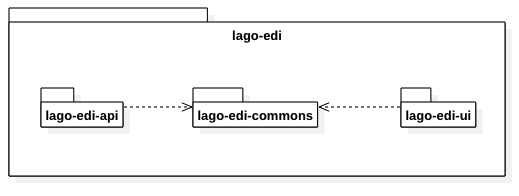
\includegraphics[scale=1, width=\textwidth]{design/general}
    \caption{Architettura generale dell'applicazione}
    \label{fig:general-design}
  \end{center}
\end{figure}

\subsection{Architettura del \emph{backend}}
In questa sezione illustro l'architettura del \emph{backend}.

\subsection{Architettura del \emph{frontend}}
In questa sezione illustro l'architettura del \emph{frontend}.

\subsection{Struttura del \emph{database}}
In questa sezione illustro la struttura del \emph{databse}.

%**************************************************************
\section{Progettazione di dettaglio}

\subsection{API per l'autenticazione}
In questa sezione descrivo le API necessarie per l'autenticazione di un utente.

\subsection{API per la manipolazione dei dati della griglia}
In questa sezione descrivo le API per la visualizzazione, la modifica e l'eliminazione dei dati della griglia.

\subsection{Diagrammi di sequenza}
In questa sezione illustro i diagrammi di sequenza relativi all'autenticazione e alla manipolazione dei dati della griglia.

%**************************************************************
\section{Codifica}

\subsection{Autenticazione}
In questa sezione illustro la porzione di codice necessaria per l'autenticazione.

\subsection{Griglia del fornitore}
In questa sezione illustro le porzioni di codice necessarie per la realizzazione della griglia del fornitore.

%**************************************************************
\section{Verifica e validazione}

\subsection{Analisi statica}
In questa sezione descrivo gli strumenti utilizzate per l'analisi statica.

\subsection{\emph{Unit Test}}
In questa sezione descrivo il framework Jest e illustro i risultati dei test effettuati con la \emph{feature code covarage}.

%**************************************************************
\section{Prodotto finale}
In questa sezione illustro le funzionalità del prodotto realizzato.